\stopallthesefloats
\subsection{METAMOC}
\begin{figure}[hbt]
\begin{center}
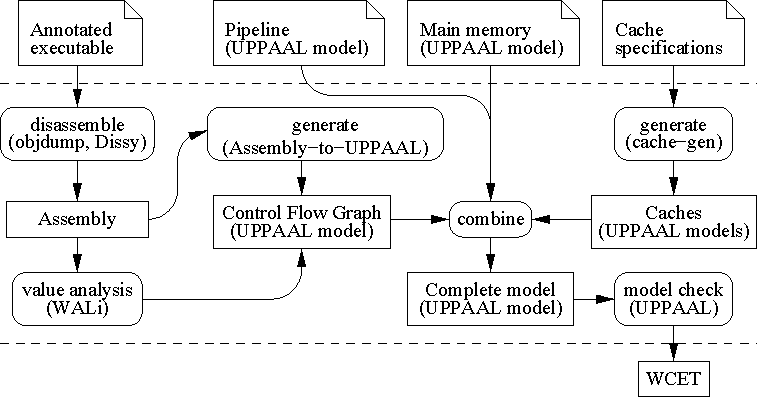
\includegraphics[width=\textwidth]{\chapterdirectory/figure/analysis/metamoc.pdf}
\end{center}
\caption{Using METAMOC to compute WCET (from
\cite{dalsgaard_et_al:OASIcs:2010:2831})}%
\label{fig:formal_analysis:metamoc}
\end{figure}

The first tool that made use of UPPAAL for the computation of WCET by modeling
hardware was Modular Execution Time Analysis using Model Checking (METAMOC),
introduced in \cite{dalsgaard_et_al:OASIcs:2010:2831}. The general idea behind
the approach is shown in Figure~\ref{fig:formal_analysis:metamoc}. The
modularity can clearly be seen in how the models for the cpu pipeline,
main memory, and cache specifications are kept separate in order to facilitate
their replacement when analyzing for a different processor. The other input is
that of the analyzed executable, directly in its binary form, albeit with some
annotations regarding loop bounds.

Given these inputs, METAMOC generates a control flow graph for the program,
which is in fact yet another UPPAAL model to combine to the ones representing
the architecture. The value analysis statically determines the address of
memory elements, and is disabled if the modeled architecture does not feature
any data cache.

The pipeline model corresponds to a collection of automata, one for each stage:
\textit{fetch}, \textit{decode}, \textit{execute}, \textit{memory}, and
\textit{writeback}. The parallel nature of pipelines translates fairly well
into a network of automata communicating through channels, making the writing
of such automata accessible for the user wanting to add their own in hopes of
modeling another architecture. The main challenges then come in determining
what can stall the pipeline on the real architecture and how long each stage
should take. Indeed, the authors of \cite{dalsgaard_et_al:OASIcs:2010:2831}
indicate that the documentation for the processor they modeled explicitly
states that it does not contain an exhaustive list of all possible stalls.

The default model for caches considers separate instructions and data caches,
matching the architecture they made their approach around. Caches are
set-associative, and implement an LRU eviction policy.

\begin{figure}[hbt!]
\begin{center}
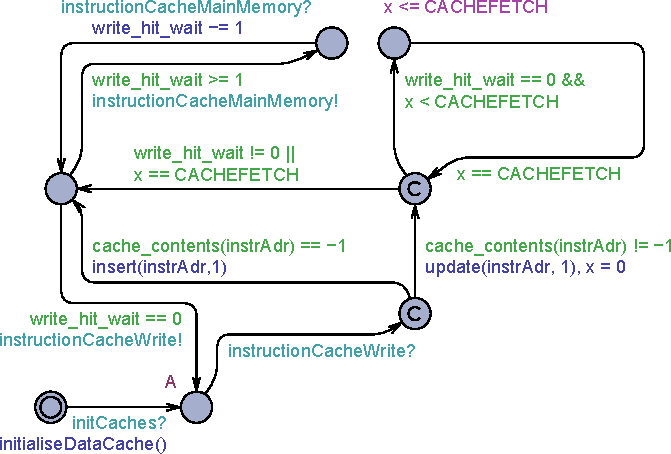
\includegraphics[width=0.8\textwidth]{\chapterdirectory/figure/analysis/half_metamoc_cache.pdf}
\end{center}
\caption{Half of Cache in METAMOC (adapted from \cite{dalsgaard_olesen_toft_2020})}%
\label{fig:formal_analysis:metamoc_caches}
\end{figure}

Figure~\ref{fig:formal_analysis:metamoc_caches} shows one half of the automaton
modeling a cache in METAMOC. The complete automaton has a second half mirroring
this one, with \textit{read} instead of write. Upon receiving a request for
a cache write, the automaton determines from its internal state whether the
request is a cache hit or if the instruction must be added to the cache. This
corresponds to \lstinline{cache_contents(instrArd)} being equal to -1 (cache
miss) or not (cache hit). In the case of a cache hit, a delay corresponding to
the time spent writing in the cache is introduced (controlled by
the \lstinline{CACHEFETCH} clock). \lstinline{write_hit_wait} corresponds to
the number of main memory accesses to be performed. Such accesses can still
occur even after a cache hit, if a write-through policy is in place. In the
case of a cache miss, a number of accesses to the main memory are performed.
This number can be higher than one if a cache line had to be evicted and the
cache follows a write-back policy. Once all accesses are performed, the cache
synchronizes on \textbf{instructionCacheWrite} to indicate that the request
was completed.

\begin{figure}[hbt!]
\begin{center}
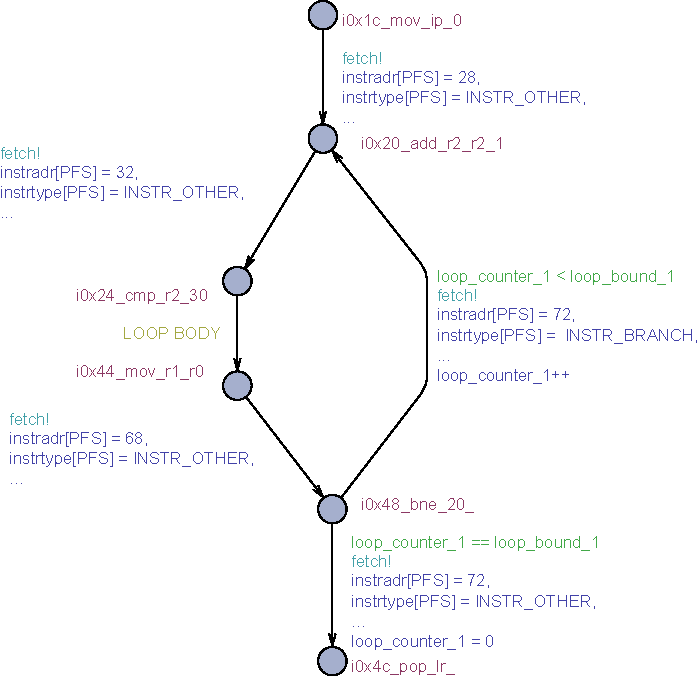
\includegraphics[width=0.8\textwidth]{\chapterdirectory/figure/analysis/metamoc_prog.pdf}
\end{center}
\caption{Fragment of Program Automaton in METAMOC (from \cite{dalsgaard_olesen_toft_2020})
}
\label{fig:formal_analysis:metamoc_program}
\end{figure}

Figure~\ref{fig:formal_analysis:metamoc_program} shows an example fragment of
an automaton corresponding to a program after processing by METAMOC. The
fragment in question corresponds to a loop, and shows how METAMOC supports
branching and iterating. The \textit{loop\_counter\_1} and
\textit{loop\_bound\_1} variables ensures that its execution terminates. The
bounds of such loops have to be annotated in the program's source code.

Their solution to limit search-space explosion is to put a caveat stating that
the architectures are assumed to be time-anomaly free, which lets them consider
only the locally worst time for some operations, instead of having to explore
all possible timings in case a better local time leads to a globally worse one.

\stopallthesefloats
